\documentclass[11pt,a4paper]{article}

\usepackage[margin=1in]{geometry}
\usepackage{graphicx}
\usepackage{booktabs}
\usepackage{longtable}
\usepackage{array}
\usepackage{xcolor}
\usepackage{hyperref}
\usepackage{caption}
\usepackage{float}

\hypersetup{
  colorlinks=true,
  linkcolor=blue,
  urlcolor=blue,
  citecolor=blue
}

\newcommand{\code}[1]{\texttt{#1}}
\newcommand{\stage}{Stage 16N}

\title{\stage{} Inhomogeneous Plate-with-Hole Cycle-Jump Benchmark\\Living Technical Report}
\author{Master Thesis Preparation}
\date{Last updated: 2026-06-07}

\begin{document}
\maketitle

\begin{abstract}
This living report records the geometry, numerical setup, HPC configuration, reference results, reinjection tests, diagnostic failures, and current conclusions for \stage{}. The stage uses an inhomogeneous Abaqus plate-with-hole benchmark with a NEML-equivalent Chaboche UMAT. The full 1000-cycle non-jump reference has been completed and is used as the validation baseline for later fixed and adaptive cycle-jump simulations. The current fixed-jump conclusion is frozen at a narrow accepted cycle-100 jump, \code{B1D5}/\code{B1D5\_EQ}: 100 $\rightarrow$ 105 $\rightarrow$ 250 with 2.34986\% maximum primary scalar-metric error. Larger and later manually initialized jumps remain blocked because \code{SDVINI}/\code{SIGINI}-based reinjection does not robustly reconstruct the later-cycle inhomogeneous finite-element state.
\end{abstract}

\tableofcontents
\newpage

\section{Purpose and Current Status}

The purpose of \stage{} is to move from single-element or homogeneous cycle-jump demonstrations to an inhomogeneous finite-element benchmark. The model is deliberately more demanding: a plate with a central hole produces localized cyclic plasticity near the hole, so the method must be judged not only from global reaction-force loops but also from local stress and state-variable evolution.

\begin{table}[H]
\centering
\caption{Current \stage{} infrastructure and validation status.}
\begin{tabular}{p{0.58\linewidth}p{0.25\linewidth}}
\toprule
Item & Status \\
\midrule
1000-cycle full non-jump reference & Completed \\
16-CPU production policy & Locked \\
Abaqus threaded launcher & Verified \\
Adaptive $\Delta N$ table & Completed \\
Exact reinjection scaffold & Prepared \\
HPC mail policy & Fixed \\
B0-1 exact reinjection solver run & Completed \\
B0-1 scientific result & Practical baseline accepted \\
B0 initialization-only audit & Completed \\
B0-2 / B0-3 exact reinjection jobs & On hold \\
Fixed state-initialized jump validation & Scaffold prepared \\
Adaptive cycle-jump workflow & On hold \\
\bottomrule
\end{tabular}
\end{table}

\section{Geometry and Model Definition}

The \stage{} model is a three-dimensional plate-with-hole benchmark. It is intended to create localized cyclic evolution near the hole while retaining a global hysteresis response that can be compared across full-reference, exact-reinjection, fixed-jump, and adaptive-jump runs.

\begin{table}[H]
\centering
\caption{Stage 16N model geometry and mesh summary.}
\begin{tabular}{ll}
\toprule
Quantity & Value \\
\midrule
Plate length & 20.0 \\
Plate height & 10.0 \\
Plate thickness & 1.0 \\
Central hole radius & 1.0 \\
Mesh spacing & $\Delta x = \Delta y = 0.25$ \\
Element type & C3D8 \\
Nodes & 6642 \\
Elements & 3148 \\
Hole-ring elements & 60 \\
Material model & NEML-equivalent Chaboche UMAT \\
State variables & 27 SDVs \\
\bottomrule
\end{tabular}
\end{table}

\begin{figure}[H]
\centering
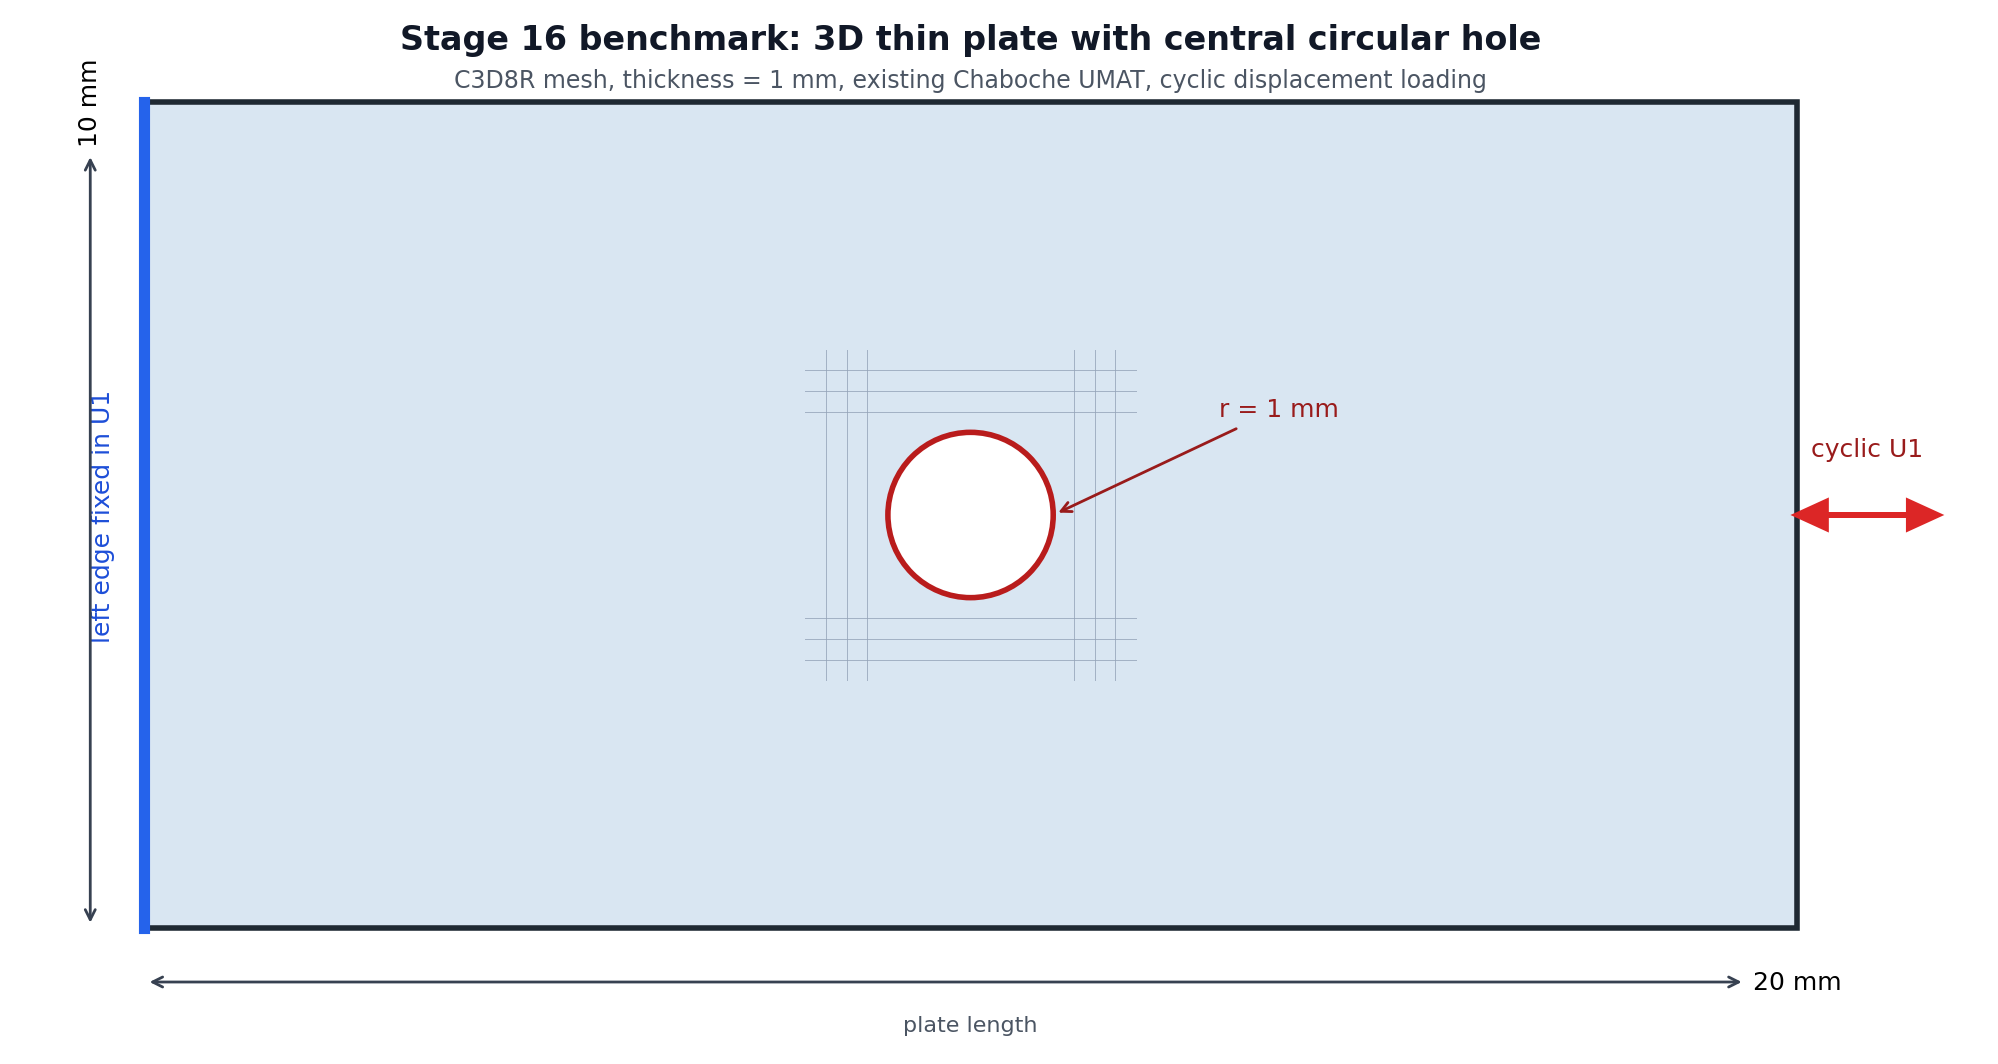
\includegraphics[width=0.82\linewidth]{figures/stage16_plate_with_hole_geometry.png}
\caption{Plate-with-hole geometry used for the \stage{} benchmark.}
\label{fig:geometry}
\end{figure}

\begin{figure}[H]
\centering
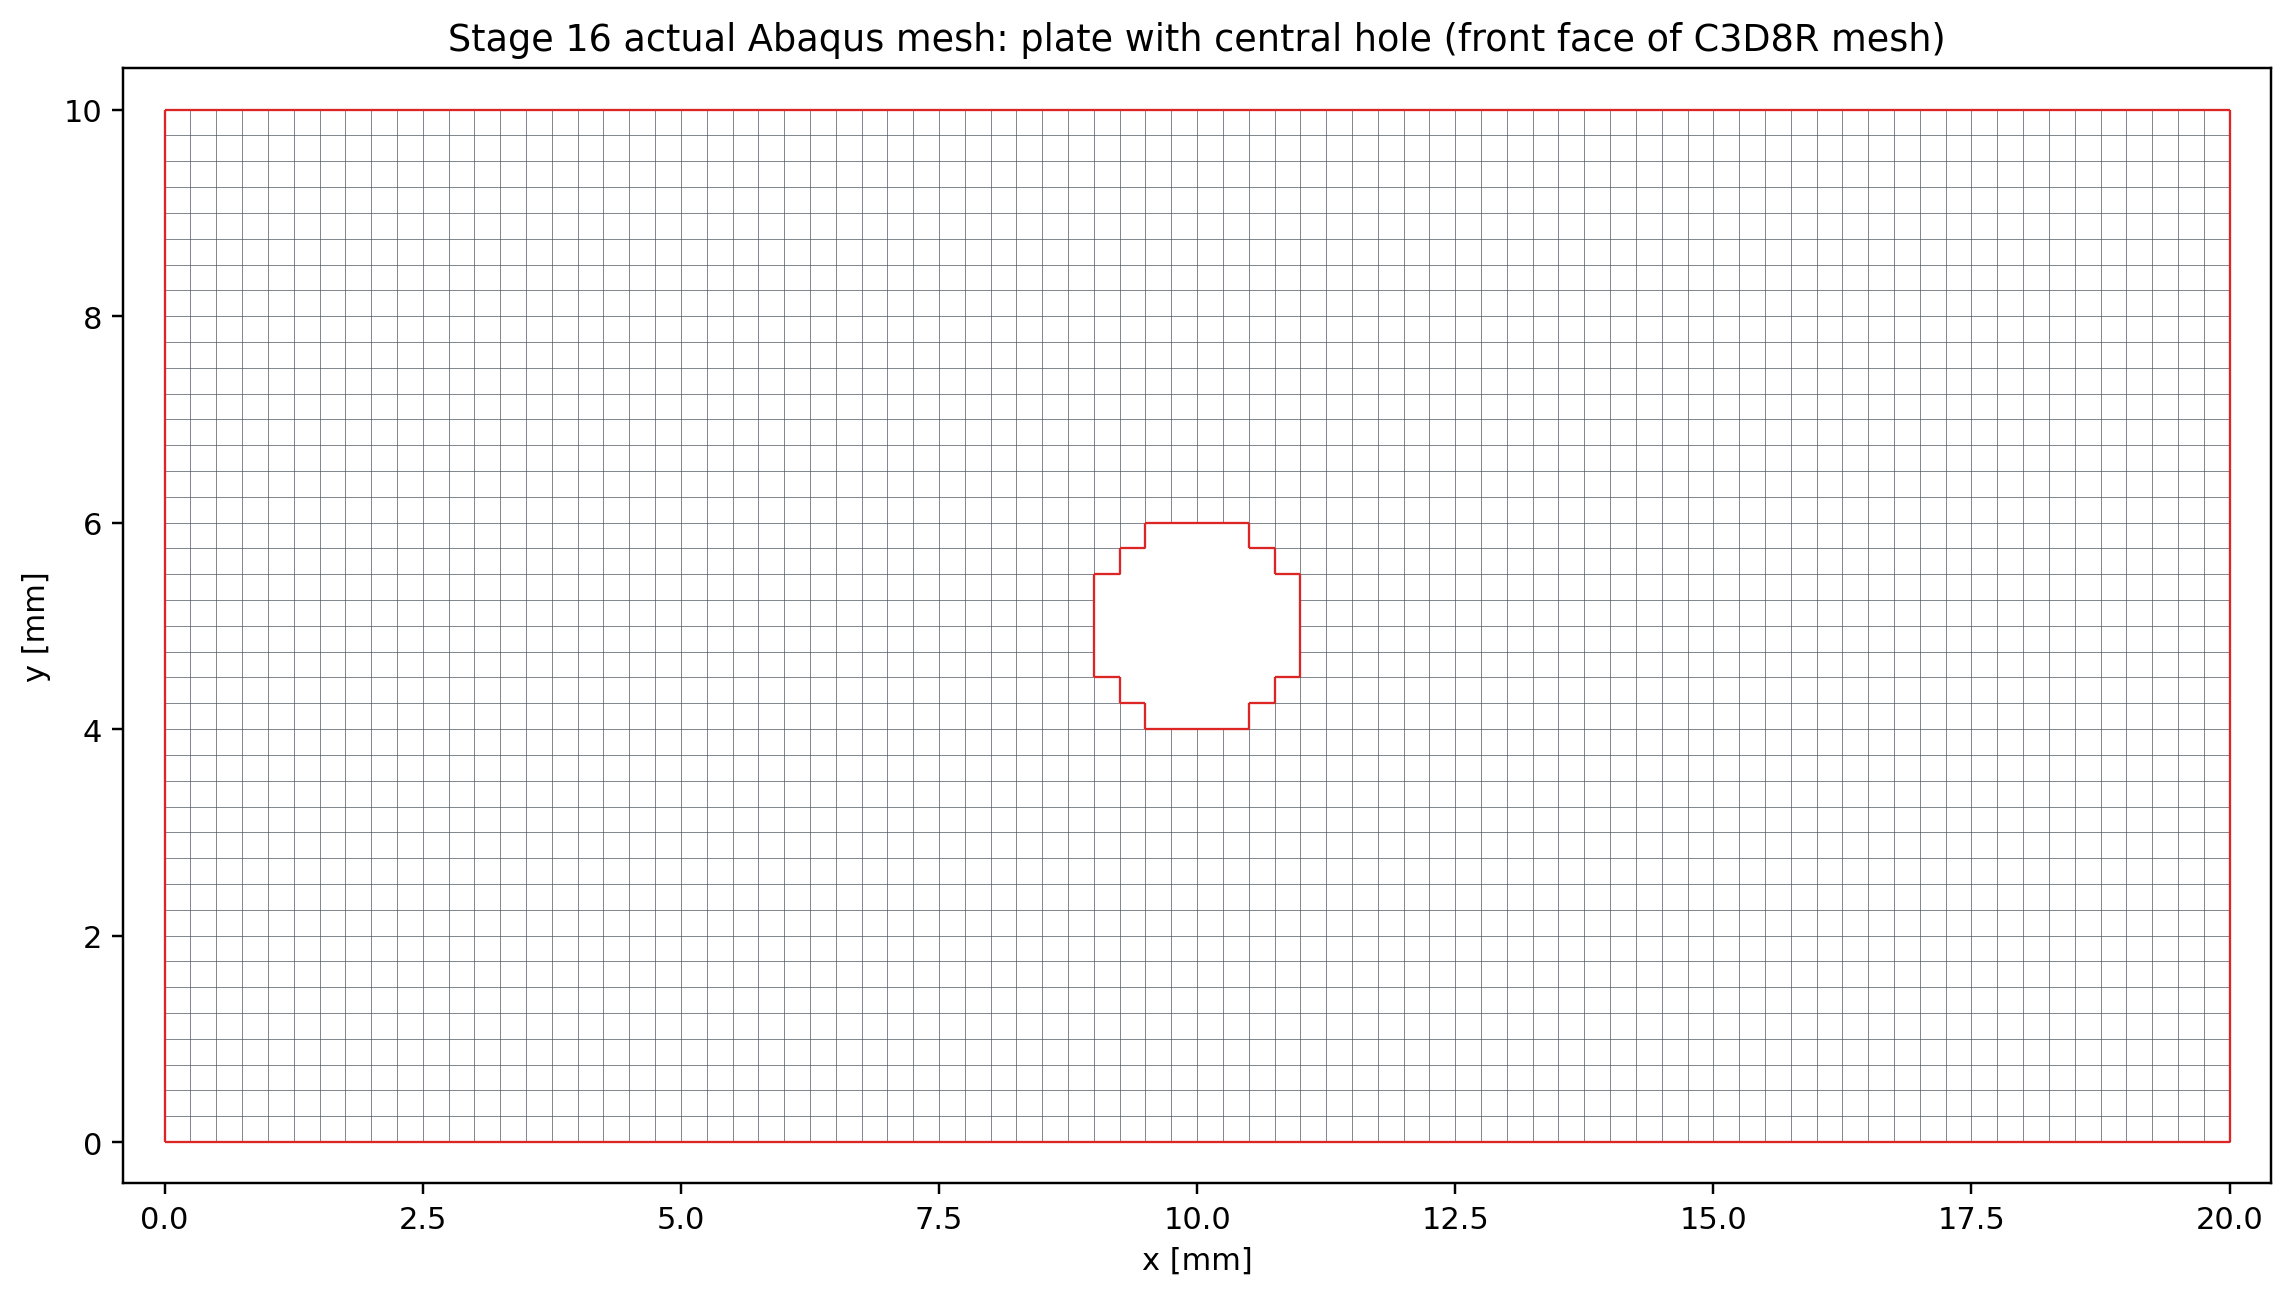
\includegraphics[width=0.82\linewidth]{figures/stage16_plate_with_hole_actual_mesh.png}
\caption{Actual structured C3D8 mesh with the element-wise approximation of the central hole.}
\label{fig:mesh}
\end{figure}

\subsection{Boundary Conditions and Loading}

The left edge is fixed in the axial direction. Two anchor nodes constrain rigid-body modes. The right edge receives a cyclic axial displacement amplitude of $\pm 0.10$. The full reference contains 1000 full non-jump cycles. Selected field output is stored at cycles 1, 2, 10, 50, 100, 250, 500, 750, and 1000.

\section{HPC and Production Policy}

The first corrected 1000-cycle parallel reference used 30 OpenMP threads, but PBS accounting showed that the average effective CPU usage was far below the requested 30 cores. A 16-CPU verification run was therefore used to lock a more resource-efficient production policy.

\begin{table}[H]
\centering
\caption{Locked \stage{} production setting.}
\begin{tabular}{ll}
\toprule
Setting & Value \\
\midrule
Production default & 1 MPI rank $\times$ 16 OpenMP threads \\
PBS request & \code{select=1:ncpus=16:mpiprocs=1:ompthreads=16} \\
Abaqus launch & \code{cpus=16 mp\_mode=threads} \\
Expected message-file line & \code{1 MPI RANK x 16 THREADS} \\
Maximum walltime per job & 24:00:00 \\
Maximum simultaneous jobs & 2 \\
Maximum active Stage 16N cores & 32 \\
\bottomrule
\end{tabular}
\end{table}

This policy is not claimed to perfectly saturate all 16 CPUs. It is a resource-efficient compromise that prevents the earlier serial fallback and avoids reserving 30 CPUs for a workload that did not use them efficiently.

\subsection{Two-Job Scheduling Policy}

From 2026-06-06 onward, \stage{} solver planning assumes at most two simultaneous production jobs. Each job requests 16 CPU cores with one MPI rank and 16 OpenMP threads, so the intended active usage is 32 CPU cores. The two slots are used only after the relevant method gate has passed. First-time method checks, such as the first fixed cycle-jump case B1, run alone until extracted and compared. If B1 passes, B2 and B3 can be submitted together. If B1 fails badly, B2 and B3 remain held and the two slots are used instead for smaller or diagnostic B1 variants.

\subsection{Mail Notification Policy}

Future PBS jobs must explicitly request mail on abort, begin, and end:

\begin{verbatim}
#PBS -m abe
#PBS -M pr21vyci@mailserver.tu-freiberg.de
\end{verbatim}

This was added because PBS accounting previously showed \code{Mail\_Points = a}, which only requests abort/failure mail.

\section{Full 1000-Cycle Non-Jump Reference}

The full non-jump reference was completed using Abaqus/Standard with the corrected threaded launcher.

\begin{table}[H]
\centering
\caption{Completed 1000-cycle reference run.}
\begin{tabular}{ll}
\toprule
Quantity & Value \\
\midrule
PBS job & 1335408.mmaster02 \\
Abaqus job & \code{stage16n\_parallel\_max\_reference\_1000cycles} \\
Walltime & 17:56:43 \\
CPU time & 178:03:42 \\
Requested resources & 30 CPUs, 135 GB \\
Abaqus parallelism & 1 MPI rank $\times$ 30 threads \\
Completed cycles & 1000 \\
Last partial cycle & none \\
\bottomrule
\end{tabular}
\end{table}

\begin{table}[H]
\centering
\caption{Reference evolution from cycle 1 to cycle 1000.}
\begin{tabular}{lrrr}
\toprule
Quantity & Cycle 1 & Cycle 1000 & Change \\
\midrule
\code{RF1\_max} & 2356.834 & 2908.244 & +23.40\% \\
\code{RF1\_min} magnitude & 2509.712 & 3074.823 & +22.52\% \\
\code{loop\_area\_abs} & 433.822 & 577.068 & +33.02\% \\
\code{HOLE\_RING\_MISES\_MAX} & 398.503 & 492.827 & +23.67\% \\
\code{HOLE\_RING\_SDV1\_MAX} & 0.0561 & 26.0519 & -- \\
\code{HOLE\_RING\_SDV8\_MAX} & 0.2996 & 92.4455 & -- \\
\code{HOLE\_RING\_SDV11\_MAX} & 7.9019 & 61.3076 & -- \\
\bottomrule
\end{tabular}
\end{table}

The evolution clearly exceeds the original continuation thresholds for global loop quantities and local hole-ring state variables. This confirms that the plate-with-hole benchmark is meaningful for cycle-jump validation.

\section{Adaptive \texorpdfstring{$\Delta N$}{Delta N} Table}

The adaptive $\Delta N$ table was computed from the completed 1000-cycle reference. It uses dense global cycle metrics and selected local field-output anchors. The controlling variable is the most sensitive monitored quantity, not only the global reaction force.

\begin{longtable}{rrrrl}
\caption{Conservative adaptive $\Delta N$ estimates from the 1000-cycle reference.}\\
\toprule
Base cycle & Next anchor & Target & $\Delta N$ & Controlling variable \\
\midrule
\endfirsthead
\toprule
Base cycle & Next anchor & Target & $\Delta N$ & Controlling variable \\
\midrule
\endhead
1 & 2 & 2 & 1 & \code{HOLE\_RING\_SDV8\_MAX} \\
2 & 10 & 3 & 1 & \code{HOLE\_RING\_SDV8\_MAX} \\
10 & 50 & 14 & 4 & \code{HOLE\_RING\_SDV8\_MAX} \\
50 & 100 & 61 & 11 & \code{HOLE\_RING\_SDV1\_MAX} \\
100 & 250 & 124 & 24 & \code{HOLE\_RING\_SDV1\_MAX} \\
250 & 500 & 299 & 49 & \code{HOLE\_RING\_SDV1\_MAX} \\
500 & 750 & 575 & 75 & \code{HOLE\_RING\_SDV1\_MAX} \\
750 & 1000 & 849 & 99 & \code{HOLE\_RING\_MISES\_MAX} \\
\bottomrule
\end{longtable}

The table shows that local state variables near the hole strongly restrict the allowable jump size. This supports the decision that any later fixed/adaptive jump validation must include local metrics, not only global RF loops.

\subsection{Reinjection-Aware Controller Update}

After the B0 initialization audit, \code{HOLE\_RING\_SDV8\_MAX} was downgraded from a hard pass/fail controller to a diagnostic-only variable because it already shows a large mismatch immediately after manual \code{SDVINI}/\code{SIGINI} initialization. A reinjection-aware table was therefore generated with \code{SDV8} retained in diagnostic output but removed from the hard controller list.

\begin{table}[H]
\centering
\caption{Reinjection-aware adaptive $\Delta N$ estimates with \code{SDV8} diagnostic-only.}
\begin{tabular}{rrrrl}
\toprule
Base & Next anchor & Target & $\Delta N$ & Controller \\
\midrule
1 & 2 & 2 & 1 & \code{HOLE\_RING\_SDV11\_MAX} \\
2 & 10 & 3 & 1 & \code{HOLE\_RING\_SDV1\_MAX} \\
10 & 50 & 15 & 5 & \code{HOLE\_RING\_SDV1\_MAX} \\
50 & 100 & 61 & 11 & \code{HOLE\_RING\_SDV1\_MAX} \\
100 & 250 & 124 & 24 & \code{HOLE\_RING\_SDV1\_MAX} \\
250 & 500 & 299 & 49 & \code{HOLE\_RING\_SDV1\_MAX} \\
500 & 750 & 575 & 75 & \code{HOLE\_RING\_SDV1\_MAX} \\
750 & 1000 & 849 & 99 & \code{HOLE\_RING\_MISES\_MAX} \\
\bottomrule
\end{tabular}
\end{table}

The first conservative fixed-jump gate remains cycle 100 to cycle 125, followed by normal continuation to cycle 250. This row is still controlled by \code{HOLE\_RING\_SDV1\_MAX}, not by diagnostic-only \code{SDV8}.

\section{Stage 16N-B: State-Initialized Continuation Verification}

Before any real cycle jump is allowed, the workflow must prove that stress and state-variable fields can be transferred into a new Abaqus run. The route used here is manual state-initialized continuation through \code{SDVINI}/\code{SIGINI}; it is not a native Abaqus restart. The originally intended verification cases were:

\begin{itemize}
  \item B0-1: exact cycle 100 state, continue normally to cycle 250.
  \item B0-2: exact cycle 250 state, continue normally to cycle 500.
  \item B0-3: exact cycle 500 state, continue normally to cycle 1000.
\end{itemize}

B0-2 and B0-3 remain on hold. The B0-1 and initialization-audit results are now treated as the measured reinjection baseline rather than as proof of an exact local restart.

\subsection{State Reader Implementation}

The initial CSV preload design failed under threaded Abaqus because multiple threads attempted to load the same file concurrently. The state-transfer implementation was therefore changed to a direct-access binary reader. Each record contains:

\begin{verbatim}
S1, S2, S3, S4, S5, S6, SDV1, ..., SDV27
\end{verbatim}

The record number is:

\begin{verbatim}
record = (NOEL - 1) * 8 + NPT
\end{verbatim}

On the Abaqus/Intel Fortran environment used here, direct-access \code{RECL} is interpreted in 4-byte words. Therefore the correct value for 33 double-precision values is:

\begin{verbatim}
RECL = 66
\end{verbatim}

\section{B0-1 Cycle-100 to Cycle-250 State-Initialized Continuation}

B0-1 completed the Abaqus solver successfully. PBS reported exit status 2 only because the original postprocessing path failed after solver completion; extraction was rerun manually afterward.

\begin{table}[H]
\centering
\caption{B0-1 run accounting and solver status.}
\begin{tabular}{ll}
\toprule
Quantity & Value \\
\midrule
PBS job & 1336497.mmaster02 \\
Route & cycle 100 state $\rightarrow$ cycle 250 \\
PBS walltime & 01:41:36 \\
PBS CPU time & 10:52:42 \\
Requested CPUs & 16 \\
Abaqus solver & completed \\
Abaqus parallelism & 1 MPI rank $\times$ 16 threads \\
Scientific status & Practical baseline accepted \\
\bottomrule
\end{tabular}
\end{table}

\begin{table}[H]
\centering
\caption{B0-1 comparison against the 1000-cycle reference at cycle 250.}
\begin{tabular}{lr}
\toprule
Quantity & Relative error \\
\midrule
\code{RF1\_max} & 0.259048\% \\
\code{RF1\_min} & 0.687538\% \\
\code{loop\_area\_abs} & 0.967300\% \\
\code{HOLE\_RING\_MISES\_MAX} & 7.63648\% \\
\code{HOLE\_RING\_S11\_MAX\_ABS} & 9.58753\% \\
\code{HOLE\_RING\_SDV1\_MAX} & 0.360172\% \\
\code{HOLE\_RING\_SDV8\_MAX} & 10.9164\% \\
\code{HOLE\_RING\_SDV11\_MAX} & 7.27213\% \\
\bottomrule
\end{tabular}
\end{table}

The global response is excellent, but the local hole-ring stress and state-variable errors are too large for a clean exact-restart claim.

\section{B0-1 Local Diagnostic Review}

A pointwise hole-ring diagnostic was run to determine whether the high local error was only a maximum-location artifact. It was not. The reference and reinjection maxima for \code{SDV8} occurred at the same element and integration point.

\begin{table}[H]
\centering
\caption{B0-1 SDV8 argmax diagnostic at cycle 250.}
\begin{tabular}{ll}
\toprule
Quantity & Value \\
\midrule
Reference SDV8 argmax & element 1242, IP 7 \\
Reinjection SDV8 argmax & element 1242, IP 7 \\
Same argmax location & true \\
Reference value & 91.1466598511 \\
Reinjection value & 81.1967315674 \\
Argmax relative error & 10.9164\% \\
\bottomrule
\end{tabular}
\end{table}

This made B0-1 a real local mismatch rather than a harmless maximum-location shift.

\section{B0 Cycle-100 Initialization-Only Audit}

The initialization audit was created to answer whether the local mismatch already exists immediately after exact cycle-100 initialization, before any cycle-100 to cycle-250 continuation.

\begin{table}[H]
\centering
\caption{Cycle-100 binary reader and initialization audit.}
\begin{tabular}{lr}
\toprule
Quantity & Value \\
\midrule
CSV-vs-binary maximum absolute error & $3.55 \times 10^{-15}$ \\
Common hole-ring element/IP records & 480 \\
\code{SDV8} median relative error & 12.7022\% \\
\code{SDV8} 95th percentile relative error & 150.665\% \\
\code{SDV8} maximum relative error & 479.090\% \\
\code{SDV8} argmax location & same element/IP, 1242/7 \\
\bottomrule
\end{tabular}
\end{table}

The binary extraction and reader pipeline is correct to machine precision. Therefore the local mismatch is not caused by the Python binary writer or direct-access file format. The mismatch appears during manual Abaqus initialization and the tiny equilibrium step.

\subsection{Initialization Audit Interpretation}

The most likely interpretation is that \code{SDVINI}/\code{SIGINI} inject stress and state variables correctly, but the manual state-initialized model does not reconstruct the compatible displacement, strain, solver-history, and full equilibrium state of the original reference analysis. Strain-like local state variables such as \code{SDV8} are therefore adjusted during the first equilibrium solve. This means B0-1 is useful as a practical state-initialized continuation test, but it is not a mathematically exact Abaqus restart for local fields.

\section{Reinjection Error Floor and Revised Metric Policy}

The B0 audit closes Stage 16N-B with the following conclusion:

\begin{quote}
Global continuation works, binary state transfer works, but local exact restart is not achieved with \code{SDVINI}/\code{SIGINI} alone.
\end{quote}

Future fixed and adaptive jump results must separate the manual reinjection error floor from the additional error caused by cycle-jump extrapolation. The primary pass/fail metrics are \code{RF1} maximum/minimum, loop area, global hysteresis shape, \code{HOLE\_RING\_SDV1\_MAX}, \code{HOLE\_RING\_SDV11\_MAX}, and \code{HOLE\_RING\_MISES\_MAX}. \code{HOLE\_RING\_S11\_MAX\_ABS} remains important, but it is now treated as a diagnostic warning metric rather than a sole hard rejection variable, because the B1D3/B1D4/B1D5 boundary study showed non-monotonic local stress sensitivity. \code{HOLE\_RING\_SDV8\_MAX} also remains diagnostic-only because it is already affected by initialization before any cycle-jump approximation is applied.

\section{Stage 16N-C Fixed State-Initialized Jump Scaffold}

Stage 16N-C now begins with one conservative fixed jump:

\begin{table}[H]
\centering
\caption{First fixed state-initialized jump case.}
\begin{tabular}{ll}
\toprule
Quantity & Value \\
\midrule
Case name & \code{B1\_100\_to\_125\_to\_250} \\
Base state & cycle 100 \\
Interpreted jump target & cycle 125 \\
Normal Abaqus continuation & cycles 126--250 \\
Comparison endpoint & cycle 250 \\
Initial state strategy & zero-order hold from cycle 100 \\
Baseline for interpretation & B0-1 cycle 100 to 250 continuation \\
\bottomrule
\end{tabular}
\end{table}

The zero-order state strategy is intentionally conservative. It measures the error added by skipping cycles 101--125 on top of the known manual reinjection floor. If this case gives acceptable global error and controlled primary local errors, the next fixed jump cases can be expanded to cycle 250 to 300, cycle 500 to 575, and cycle 750 to 850.

\subsection{Prepared-Only B2 and B3 Cases}

B2 and B3 may be prepared while B1 is running, but their solver jobs are gated by the B1 result. They must not be submitted until B1 has been extracted, compared against the 1000-cycle reference, and interpreted against the B0 reinjection baseline.

\begin{table}[H]
\centering
\caption{Prepared-only fixed-jump cases held behind the B1 gate.}
\begin{tabular}{llll}
\toprule
Case & Base state & Jump target & Compare endpoint \\
\midrule
\code{B2\_250\_to\_300\_to\_500} & cycle 250 & cycle 300 & cycle 500 \\
\code{B3\_500\_to\_575\_to\_750} & cycle 500 & cycle 575 & cycle 750 \\
\bottomrule
\end{tabular}
\end{table}

If B1 passes, B2 and B3 are the first paired submission under the new two-job policy. If B1 fails, the paired slots should instead be used for B1-small and B1-diagnostic variants.

\subsection{B1 Result}

B1 completed successfully as an Abaqus job, but it did not pass the fixed-jump method gate. The comparison at cycle 250 gave good global errors but unacceptable primary local state errors.

\begin{table}[H]
\centering
\caption{B1 fixed-jump comparison against the 1000-cycle reference and B0 baseline.}
\begin{tabular}{lrrr}
\toprule
Quantity & B1 total error & B0 baseline & Additional error \\
\midrule
\code{RF1\_max} & 0.361433\% & 0.259048\% & 0.102384\% \\
\code{RF1\_min} & 2.27018\% & 0.687538\% & 1.58264\% \\
\code{loop\_area\_abs} & 1.26223\% & 0.967300\% & 0.294934\% \\
\code{HOLE\_RING\_MISES\_MAX} & 2.40141\% & 7.63648\% & -5.23507\% \\
\code{HOLE\_RING\_S11\_MAX\_ABS} & 1.21869\% & 9.58753\% & -8.36884\% \\
\code{HOLE\_RING\_SDV1\_MAX} & 10.2916\% & 0.360172\% & 9.93139\% \\
\code{HOLE\_RING\_SDV8\_MAX} & 16.1769\% & 10.9164\% & 5.26047\% \\
\code{HOLE\_RING\_SDV11\_MAX} & 11.2777\% & 7.27213\% & 4.00560\% \\
\bottomrule
\end{tabular}
\end{table}

The B1 status is \code{review}, controlled by \code{HOLE\_RING\_SDV11\_MAX}. Therefore B2 and B3 remain held. The two-job policy should next be used for smaller or diagnostic B1 variants rather than larger fixed jumps.

\subsection{B1 Jump-Size Sensitivity}

The next two-job batches reduced the first fixed jump from cycle 100 to smaller target cycles while keeping the same comparison endpoint at cycle 250. This directly tests whether the local hole-ring error decreases when fewer cycles are skipped.

\begin{table}[H]
\centering
\caption{B1 fixed-jump sensitivity at cycle 250.}
\begin{tabular}{lrrll}
\toprule
Case & Jump target & Skipped cycles & Status & Controlling quantity \\
\midrule
\code{B1Q\_100\_to\_106\_to\_250} & 106 & 6 & review, 5.75372\% & \code{HOLE\_RING\_MISES\_MAX} \\
\code{B1S\_100\_to\_112\_to\_250} & 112 & 12 & review, 9.34203\% & \code{HOLE\_RING\_S11\_MAX\_ABS} \\
\code{B1\_100\_to\_125\_to\_250} & 125 & 25 & review, 11.2777\% & \code{HOLE\_RING\_SDV11\_MAX} \\
\bottomrule
\end{tabular}
\end{table}

The sensitivity study confirms that the original jump from cycle 100 to 125 was too aggressive for local hole-ring variables. Reducing the target to cycle 106 reduced the maximum primary error to approximately 5.75\%, but this remained above the strict 5\% gate. The useful scientific conclusion is that the adaptive jump-size estimate near cycle 100 was too optimistic and must be reduced by an early-cycle safety factor. Since the reinjection-aware table suggested approximately $\Delta N \approx 24$ at cycle 100, the practical early safety factor is approximately

\[
  \frac{5}{24} \approx 0.21 .
\]

This supports an early-cycle safety-factor range of approximately 0.20--0.25, controlled by local field quantities rather than by \code{RF1} alone.

\subsection{B1D3/B1D4/B1D5 Boundary Check}

A stricter boundary check was then performed with target cycles 103, 104, and 105. The result is useful, but non-monotonic:

\begin{table}[H]
\centering
\caption{B1D3/B1D4/B1D5 boundary check at cycle 250.}
\begin{tabular}{lrrll}
\toprule
Case & Jump target & Skipped cycles & Status & Controlling quantity \\
\midrule
\code{B1D3\_100\_to\_103\_to\_250} & 103 & 3 & review, 9.13095\% & \code{HOLE\_RING\_S11\_MAX\_ABS} \\
\code{B1D4\_100\_to\_104\_to\_250} & 104 & 4 & review, 9.34307\% & \code{HOLE\_RING\_S11\_MAX\_ABS} \\
\code{B1D5\_100\_to\_105\_to\_250} & 105 & 5 & pass, 2.34986\% & \code{HOLE\_RING\_SDV1\_MAX} \\
\code{B1Q\_100\_to\_106\_to\_250} & 106 & 6 & review, 5.75372\% & \code{HOLE\_RING\_MISES\_MAX} \\
\bottomrule
\end{tabular}
\end{table}

B1D5 remains a useful successful case:

\begin{quote}
\code{100 -> 105 -> 250}, with maximum primary error 2.34986\%.
\end{quote}

However, B1D3 and B1D4 both failed under the local stress criterion even though they used shorter jumps. B1D3 was controlled by \code{HOLE\_RING\_S11\_MAX\_ABS} at 9.13095\%, and B1D4 was controlled by the same metric at 9.34307\%. Therefore the cycle-100 boundary is not robust under a hard local-stress maximum criterion. The isolated B1D5 pass should not be generalized as a universal accepted early-cycle rule.

\subsection{B1D4 Pointwise Diagnostic}

B1D4 was diagnosed at the hole-ring element/integration-point level using the 1000-cycle reference ODB and the B1D4 ODB at cycle 250. The diagnostic compared 480 common hole-ring element/IP records and checked both pointwise errors and argmax locations.

\begin{table}[H]
\centering
\caption{B1D4 pointwise diagnostic summary at cycle 250.}
\begin{tabular}{lrrrr}
\toprule
Variable & Mean error & Median error & 95th percentile & Max pointwise error \\
\midrule
\code{S11\_ABS} & 13.8050\% & 11.6186\% & 35.2953\% & 121.4232\% \\
\code{MISES} & 8.05921\% & -- & -- & -- \\
\code{SDV1} & 1.64737\% & -- & -- & -- \\
\code{SDV8} & 131.337\% & -- & -- & -- \\
\code{SDV11} & 50.4912\% & -- & -- & -- \\
\bottomrule
\end{tabular}
\end{table}

For the controlling stress metric, the reference and B1D4 argmax location were the same:

\begin{quote}
\code{S11\_ABS} argmax element/IP = \code{1242/7} in both the reference and B1D4.
\end{quote}

The global phase check did not show a cycle-phase mismatch. Both runs used \code{CYCLE\_0250}; the cycle had local time from 0 to 1, displacement extrema matched exactly, and the global loop-area error was only 0.107074\%. Therefore the B1D4 failure is not explained by a simple output-phase or step-numbering mismatch. It appears to be a real local stress/reinjection sensitivity in the B1D4 path.

This keeps the conservative decision unchanged: B1D5 is a useful pass case, but B1D3 and B1D4 show that the early-cycle jump boundary is not robust when local stress extrema are treated as hard primary rejection variables.

\subsection{B1D3 Confirmation Result}

B1D3 completed successfully as an Abaqus job and was compared against the 1000-cycle reference at cycle 250. It did not pass the fixed-jump gate.

\begin{table}[H]
\centering
\caption{B1D3 comparison against the 1000-cycle reference at cycle 250.}
\begin{tabular}{lr}
\toprule
Quantity & Relative error \\
\midrule
\code{RF1\_max} & 1.45771\% \\
\code{RF1\_min} & 0.661665\% \\
\code{loop\_area\_abs} & 0.214351\% \\
\code{HOLE\_RING\_MISES\_MAX} & 7.43637\% \\
\code{HOLE\_RING\_S11\_MAX\_ABS} & 9.13095\% \\
\code{HOLE\_RING\_SDV1\_MAX} & 1.52456\% \\
\code{HOLE\_RING\_SDV8\_MAX} & 9.68802\% \\
\code{HOLE\_RING\_SDV11\_MAX} & 5.43394\% \\
\bottomrule
\end{tabular}
\end{table}

B1D3 confirms that the B1D4 behavior is not an isolated single-case artifact. The global response remains accurate, but the local hole-ring stress maximum and \code{SDV11} response exceed the strict local threshold. The current interpretation is therefore:

\begin{quote}
Early-cycle jumping from cycle 100 is not robust under local stress-maximum acceptance. The pass at cycle 105 is useful evidence that small jumps can work, but the non-monotonic failures at cycles 103 and 104 require a more careful local acceptance strategy or a later-start jump strategy.
\end{quote}

\subsection{Revised Local-Stress Acceptance Policy}

The B1D3/B1D4/B1D5 boundary is scientifically important because it shows that smaller jumps are not always better when judged by a single local stress maximum. The robust conclusion is:

\begin{quote}
Global hysteresis quantities are robust, but local stress-maximum metrics near the hole are non-monotonic and highly sensitive to manual state initialization and re-equilibration.
\end{quote}

Therefore, \code{HOLE\_RING\_S11\_MAX\_ABS} is retained and reported, but it should not be used as the only hard pass/fail metric. The revised three-level metric strategy is:

\begin{itemize}
  \item Primary pass/fail: \code{RF1} extrema, loop area, \code{HOLE\_RING\_SDV1\_MAX}, \code{HOLE\_RING\_SDV11\_MAX}, and \code{HOLE\_RING\_MISES\_MAX}.
  \item Secondary/diagnostic: \code{HOLE\_RING\_S11\_MAX\_ABS}, single-point stress maxima, and \code{SDV8}.
  \item Robust local-field additions: mean/median, 95th percentile, or 99th percentile hole-ring stress errors from pointwise distributions.
\end{itemize}

This does not hide the local stress sensitivity. It reports it as evidence that local extrema are more restrictive and less stable than global hysteresis metrics.

The current reporting conclusion is:

\begin{quote}
The B1 sensitivity study showed that the original jump from cycle 100 to 125 was too aggressive for the local hole-ring variables. Reducing the jump to cycle 105 gave an acceptable maximum primary error of 2.35\%, but the cycle 103 and 104 cases both produced non-monotonic local stress errors controlled by \code{HOLE\_RING\_S11\_MAX\_ABS}. Therefore, early-cycle jumping from cycle 100 cannot yet be accepted as robust under a hard local stress-maximum criterion.
\end{quote}

B2 and B3 remain held. The next two-job policy is therefore used for one smaller cycle-100 diagnostic jump and one later-cycle safe pilot, rather than for the original larger fixed jumps.

\begin{table}[H]
\centering
\caption{Next two-job diagnostic pair submitted after the B1D3 result.}
\begin{tabular}{lllll}
\toprule
Case & Route & Purpose & PBS job & Status at submission \\
\midrule
\code{B1D2\_100\_to\_102\_to\_250} & 100 $\rightarrow$ 102 $\rightarrow$ 250 & cycle-100 hard-stress check & 1341026.mmaster02 & running \\
\code{B2SAFE\_250\_to\_260\_to\_500} & 250 $\rightarrow$ 260 $\rightarrow$ 500 & later-start safe pilot & 1341027.mmaster02 & failed in equilibration \\
\code{B2SAFE\_EQ\_250\_to\_260\_to\_500} & 250 $\rightarrow$ 260 $\rightarrow$ 500 & smaller equilibration increment & 1341028.mmaster02 & failed in equilibration \\
\bottomrule
\end{tabular}
\end{table}

The first B2SAFE submission failed after datacheck during \code{FIXED\_JUMP\_EQUILIBRATE\_TO\_CYCLE\_0260}. Abaqus reported slow force convergence and \code{TOO MANY ATTEMPTS MADE FOR THIS INCREMENT}. A distinct rerun case, \code{B2SAFE\_EQ\_250\_to\_260\_to\_500}, reduced the equilibration initial increment from $1.0 \times 10^{-6}$ to $1.0 \times 10^{-8}$, but it failed in the same first equilibration step after cutbacks to $6.25 \times 10^{-10}$. This is a useful result by itself: the later cycle-250 reinjection point is numerically more difficult to equilibrate than the cycle-100 cases, and it requires an explicit cycle-250 reinjection/equilibration diagnostic before B2-safe can be interpreted scientifically.

\subsection{Unattended Dependency Queue}

The unattended queue was reorganized into two dependency-controlled streams so that at most two 16-CPU jobs can run at once while preserving the scientific gates.

\begin{table}[H]
\centering
\caption{Dependency-controlled unattended queue.}
\begin{tabular}{llll}
\toprule
Stream & Case & PBS job & Dependency/status \\
\midrule
A & \code{B1D2\_100\_to\_102\_to\_250} & 1341026.mmaster02 & running \\
A & \code{B1D1\_100\_to\_101\_to\_250} & 1341029.mmaster02 & \code{afterany:1341026} \\
B & \code{B0\_250\_to\_500} & 1341033.mmaster02 & failed in reinjection equilibration \\
B & \code{B2D2\_250\_to\_252\_to\_500} & 1341034.mmaster02 & afterok not satisfied \\
B & \code{B2D5\_250\_to\_255\_to\_500} & 1341035.mmaster02 & afterok not satisfied \\
B & \code{B0\_AUDIT\_0250\_INITIALIZATION\_ONLY} & 1341036.mmaster02 & failed in equilibration \\
\bottomrule
\end{tabular}
\end{table}

The first B0-2 exact-reinjection submission, 1341030.mmaster02, exited with status 126 because the PBS script had CRLF line endings and invoked \code{/bin/bash\string^M}. Its dependent jobs 1341031 and 1341032 did not run as meaningful solver jobs. The exact-reinjection submit writer was corrected to write LF-only PBS scripts, the remote PBS file was normalized, and Stream B was resubmitted as jobs 1341033--1341035.

The corrected B0-2 job, 1341033.mmaster02, then ran Abaqus and failed during the first \code{REINJECTION\_EQUILIBRATE} increment with \code{TOO MANY ATTEMPTS MADE FOR THIS INCREMENT}. Therefore B2D2 and B2D5 correctly remained blocked by their \code{afterok} dependencies. The Stream B replacement, \code{B0\_AUDIT\_0250\_INITIALIZATION\_ONLY} job 1341036.mmaster02, also failed in its first initialization/equilibration increment after cutbacks to $6.25 \times 10^{-11}$. This means the cycle-250 problem is not a jump-size result: exact cycle-250 manual state injection cannot yet be equilibrated robustly.

\subsection{Long-Weekend Dependency Extension}

Because the user will be away for more than 40 hours, the unattended queue was extended with additional scientifically safe diagnostics. The queue still preserves the two-job policy: only one Stream A job and one Stream B job can run at a time, and every job requests 16 CPUs, 90 GB, and 24 hours.

\begin{table}[H]
\centering
\caption{Extended long-weekend queue.}
\begin{tabular}{llll}
\toprule
Stream & Case & PBS job & Dependency/status \\
\midrule
A & \code{B1D2\_100\_to\_102\_to\_250} & 1341026.mmaster02 & running \\
A & \code{B1D1\_100\_to\_101\_to\_250} & 1341029.mmaster02 & \code{afterany:1341026} \\
A & \code{B1D2\_EQ\_100\_to\_102\_to\_250} & 1341037.mmaster02 & \code{afterany:1341029} \\
A & \code{B1D1\_EQ\_100\_to\_101\_to\_250} & 1341038.mmaster02 & \code{afterany:1341037} \\
B & \code{B0\_AUDIT\_0500\_INITIALIZATION\_ONLY} & 1341039.mmaster02 & running \\
B & \code{B0\_AUDIT\_0250\_SDVINI\_ONLY} & 1341040.mmaster02 & \code{afterany:1341039} \\
B & \code{B0\_AUDIT\_0250\_SIGINI\_ONLY} & 1341041.mmaster02 & \code{afterany:1341040} \\
B & \code{B0\_AUDIT\_0500\_SDVINI\_ONLY} & 1341042.mmaster02 & \code{afterany:1341041} \\
B & \code{B0\_AUDIT\_0500\_SIGINI\_ONLY} & 1341043.mmaster02 & \code{afterany:1341042} \\
\bottomrule
\end{tabular}
\end{table}

The two \code{B1D*\_EQ} jobs are fallback diagnostics with a smaller equilibration initial increment. They should be interpreted as numerical sensitivity checks for the cycle-100 boundary, not as authorization to submit B2/B3. The Stream B audit jobs split the manual cycle-250 and cycle-500 state injection into full, \code{SDVINI}-only, and \code{SIGINI}-only variants. This should identify whether the cycle-250/500 equilibration barrier is driven primarily by STATEV injection, stress injection, or the coupled manual restart.

The Stream B injection-only diagnostics completed quickly and all returned exit status 1. Therefore, a second B1-only EQ stream was submitted into the free slot. This keeps the cluster at the intended two active 16-core jobs while continuing to avoid B2/B3.

\begin{table}[H]
\centering
\caption{Final long-weekend live and queued jobs.}
\begin{tabular}{llll}
\toprule
Stream & Case & PBS job & Dependency/status \\
\midrule
A & \code{B1D2\_100\_to\_102\_to\_250} & 1341026.mmaster02 & running \\
A & \code{B1D1\_100\_to\_101\_to\_250} & 1341029.mmaster02 & \code{afterany:1341026} \\
A & \code{B1D2\_EQ\_100\_to\_102\_to\_250} & 1341037.mmaster02 & \code{afterany:1341029} \\
A & \code{B1D1\_EQ\_100\_to\_101\_to\_250} & 1341038.mmaster02 & \code{afterany:1341037} \\
A & \code{B1D3\_EQ\_100\_to\_103\_to\_250} & 1341044.mmaster02 & \code{afterany:1341038} \\
A & \code{B1D4\_EQ\_100\_to\_104\_to\_250} & 1341045.mmaster02 & \code{afterany:1341044} \\
A & \code{B1D5\_EQ\_100\_to\_105\_to\_250} & 1341046.mmaster02 & \code{afterany:1341045} \\
C & \code{B1Q\_EQ\_100\_to\_106\_to\_250} & 1341047.mmaster02 & running \\
C & \code{B1S\_EQ\_100\_to\_112\_to\_250} & 1341048.mmaster02 & \code{afterany:1341047} \\
C & \code{B1\_EQ\_100\_to\_125\_to\_250} & 1341049.mmaster02 & \code{afterany:1341048} \\
\bottomrule
\end{tabular}
\end{table}

The final live/queued solver count after this extension was 10 jobs: 2 running and 8 held by dependencies. The active requested resource load was therefore $2 \times 16 = 32$ CPU cores.

\subsection{Post-Queue Check on 2026-06-07}

The long-weekend queue had drained by the 2026-06-07 check: \code{qstat -u pr21vyci} returned no active jobs. The PBS extended-history query with \code{qstat -x -f} no longer exposed the listed job IDs, returning \code{Unknown Job Id} for 1341026, 1341029, 1341037, 1341038, 1341044--1341049, and the audit jobs 1341039--1341043. Therefore the final job assessment below is based on the completed run artifacts in the remote Stage 16N directory and the refreshed comparison CSVs, not on retained PBS accounting records.

\begin{table}[H]
\centering
\caption{Final fixed-jump comparison after the dependency queue drained.}
\begin{tabular}{lllll}
\toprule
Case & Route & Status & Max primary error & Controller \\
\midrule
\code{B1D1} & 100 $\rightarrow$ 101 $\rightarrow$ 250 & review & 8.70868\% & \code{SDV11} \\
\code{B1D1\_EQ} & 100 $\rightarrow$ 101 $\rightarrow$ 250 & review & 8.70868\% & \code{SDV11} \\
\code{B1D2} & 100 $\rightarrow$ 102 $\rightarrow$ 250 & review & 8.79420\% & \code{SDV11} \\
\code{B1D2\_EQ} & 100 $\rightarrow$ 102 $\rightarrow$ 250 & review & 8.79420\% & \code{SDV11} \\
\code{B1D3} & 100 $\rightarrow$ 103 $\rightarrow$ 250 & review & 7.43637\% & \code{MISES} \\
\code{B1D3\_EQ} & 100 $\rightarrow$ 103 $\rightarrow$ 250 & review & 7.43637\% & \code{MISES} \\
\code{B1D4} & 100 $\rightarrow$ 104 $\rightarrow$ 250 & review & 7.54718\% & \code{SDV11} \\
\code{B1D4\_EQ} & 100 $\rightarrow$ 104 $\rightarrow$ 250 & review & 7.54718\% & \code{SDV11} \\
\code{B1D5} & 100 $\rightarrow$ 105 $\rightarrow$ 250 & pass & 2.34986\% & \code{SDV1} \\
\code{B1D5\_EQ} & 100 $\rightarrow$ 105 $\rightarrow$ 250 & pass & 2.34986\% & \code{SDV1} \\
\code{B1Q} & 100 $\rightarrow$ 106 $\rightarrow$ 250 & review & 5.75372\% & \code{MISES} \\
\code{B1Q\_EQ} & 100 $\rightarrow$ 106 $\rightarrow$ 250 & review & 5.75372\% & \code{MISES} \\
\code{B1S} & 100 $\rightarrow$ 112 $\rightarrow$ 250 & review & 7.63033\% & \code{SDV11} \\
\code{B1S\_EQ} & 100 $\rightarrow$ 112 $\rightarrow$ 250 & review & 7.63033\% & \code{SDV11} \\
\code{B1} & 100 $\rightarrow$ 125 $\rightarrow$ 250 & review & 11.27770\% & \code{SDV11} \\
\code{B1\_EQ} & 100 $\rightarrow$ 125 $\rightarrow$ 250 & review & 11.27770\% & \code{SDV11} \\
\bottomrule
\end{tabular}
\end{table}

The smaller-equilibration \code{EQ} reruns reproduced the same comparison errors as their non-\code{EQ} counterparts. This is important: the cycle-100 B1 jump-size trend is controlled by the physical/local state mismatch relative to the 1000-cycle reference, not by the initial equilibration increment used in the fixed-jump continuation. Under the current 5\% primary-error gate, only the 100 $\rightarrow$ 105 $\rightarrow$ 250 case passes; the 100 $\rightarrow$ 106 and larger jumps remain above threshold, and the 100 $\rightarrow$ 101/102/103/104 cases still show local-state or Mises review errors.

The later-cycle fixed-jump candidates \code{B2}, \code{B2SAFE}, \code{B2SAFE\_EQ}, \code{B2D2}, \code{B2D5}, and \code{B3} remain \code{missing\_outputs}. This is expected because the cycle-250 exact-reinjection/equilibration gate failed and the unsafe dependent jobs were not allowed to produce accepted fixed-jump validations.

\subsection{Robust Scalar-Metric Re-score}

The completed B1/B1\_EQ family was re-scored with robust scalar statistics: mean, median, 95th percentile, 99th percentile, and maximum relative error. This re-score uses the lightweight scalar metrics retained in the repository. It is not yet a full pointwise field-percentile study because complete per-integration-point fields were not retained for every B1 case. Loop errors were normalized by the full reference loop amplitude for \code{U1\_avg} and \code{RF1\_sum}, avoiding artificial blow-ups at zero crossings.

\begin{table}[H]
\centering
\caption{Robust scalar-metric re-score for representative B1 cases.}
\begin{tabular}{lrrrrrl}
\toprule
Case & Mean & Median & p95 & p99 & Max & Status \\
\midrule
\code{B1D1} & 2.97163\% & 1.77699\% & 7.47991\% & 8.46293\% & 8.70868\% & review \\
\code{B1D3} & 2.78810\% & 1.49114\% & 6.93576\% & 7.33625\% & 7.43637\% & review \\
\code{B1D5} & 0.392238\% & 0.000247\% & 1.76313\% & 2.23251\% & 2.34986\% & pass by max \\
\code{B1D5\_EQ} & 0.392238\% & 0.000247\% & 1.76313\% & 2.23251\% & 2.34986\% & pass by max \\
\code{B1Q} & 2.54352\% & 2.34673\% & 4.99948\% & 5.60287\% & 5.75372\% & robust pass, max review \\
\code{B1Q\_EQ} & 2.54352\% & 2.34673\% & 4.99948\% & 5.60287\% & 5.75372\% & robust pass, max review \\
\code{B1S} & 3.65193\% & 3.12240\% & 7.50946\% & 7.60616\% & 7.63033\% & review \\
\code{B1} & 4.64409\% & 2.33580\% & 11.0312\% & 11.2284\% & 11.2777\% & review \\
\bottomrule
\end{tabular}
\end{table}

The robust scalar re-score supports the same conservative conclusion as the hard maximum-error gate. \code{B1D5} and \code{B1D5\_EQ} are the only clean passes. \code{B1Q} and \code{B1Q\_EQ} are scientifically interesting because their primary p95 error is just below 5\%, but their maxima still exceed the 5\% gate. Therefore they should be treated as borderline review cases unless a later full-field percentile acceptance rule is deliberately adopted.

\subsection{Limitations of Manual SDVINI/SIGINI Reinjection}

The later-cycle diagnostics show that the bottleneck is no longer only jump size. Manual \code{SDVINI}/\code{SIGINI} reinjection starts a scratch Abaqus model with injected stress and state variables, but it does not preserve the compatible displacement field, strain field, equilibrium state, solver history, or tangent/history information of the original inhomogeneous analysis. At cycle 100 this route is good enough for a narrow global-response demonstration. At cycle 250 and cycle 500 it failed before valid physical continuation in exact, \code{SDVINI}-only, \code{SIGINI}-only, and combined diagnostics.

This is a thesis-useful limitation result: manual state initialization is not robust enough for later-cycle reinjection in the plate-with-hole benchmark. Repeating B2/B3 jobs with the same scratch \code{SDVINI}/\code{SIGINI} route is therefore not expected to add scientific value. The next path is Stage 16N-R, a reinjection-strategy repair that preserves Abaqus' finite-element state through native restart or in-analysis continuation and applies the cycle jump only to independent material memory variables.

\section{Failures and Fixes}

\begin{longtable}{p{0.26\linewidth}p{0.34\linewidth}p{0.32\linewidth}}
\caption{Important failures and fixes recorded in \stage{}.}\\
\toprule
Issue & Observation & Fix / conclusion \\
\midrule
\endfirsthead
\toprule
Issue & Observation & Fix / conclusion \\
\midrule
\endhead
Accidental serial-like run & A 22-hour run reached only 592 full cycles. & Parallel launcher corrected; later 1000-cycle reference completed. \\
30-CPU over-allocation & 30-thread run averaged about 10 effective cores. & 16 CPUs selected as production compromise. \\
Missing start/end email & PBS accounting showed \code{Mail\_Points = a}. & Added \code{\#PBS -m abe} and mail user to Stage 16N submit scripts. \\
CSV state-reader race & Threaded Abaqus calls attempted concurrent CSV preload. & Replaced with direct-access binary state reader. \\
Wrong direct-access record length & Abaqus/Intel runtime expected word-based \code{RECL}. & Set \code{RECL = 66} for 33 double values. \\
Postprocessing path failure & B0-1 solver completed but PBS exit status was 2. & Fixed extractor path and reran extraction manually. \\
B0-1 local mismatch & Global errors under 1\%, local \code{SDV8} max error 10.9164\%. & Added pointwise diagnostic and initialization-only audit. \\
Initialization local mismatch & Binary audit passed, but \code{SDV8} mismatch appeared immediately. & Concluded manual \code{SDVINI}/\code{SIGINI} is not a mathematically exact local restart. \\
Metric policy mismatch & Original adaptive table allowed \code{SDV8} to act as a hard controller. & Added reinjection-aware table with \code{SDV8} diagnostic-only. \\
B1 fixed-jump gate & Global B1 errors were small, but \code{SDV1} and \code{SDV11} primary local errors exceeded 10\%. & Hold B2/B3 and use the two-job policy for smaller/debug B1 variants. \\
B1D4/B1D5 non-monotonic boundary & B1D5 passed at 2.34986\%, but B1D4 failed at 9.34307\% controlled by \code{S11}. & Accept \code{100 -> 105} only with diagnostic confirmation; diagnose B1D4 before B2/B3. \\
B1D4 pointwise diagnostic & B1D4 and the reference share the same \code{S11\_ABS} argmax location, and median/p95 stress errors are not negligible. & Treat B1D4 as real local stress sensitivity, not a simple phase or argmax-swap artifact. \\
B1D3 confirmation & B1D3 also failed at 9.13095\%, controlled by \code{S11\_ABS}. & Do not generalize the B1D5 pass; treat cycle-100 jumping as not robust under hard local stress maxima. \\
Metric policy revision & \code{S11\_MAX\_ABS} is non-monotonic across B1D3/B1D4/B1D5. & Keep \code{S11} maxima as diagnostic warnings; use global, STATEV, and Mises-type metrics as primary acceptance controls. \\
Completed B1 dependency queue & The drained queue shows \code{B1D5} and \code{B1D5\_EQ} pass at 2.34986\%, while all other completed B1-size variants remain review cases. & Treat 100 $\rightarrow$ 105 $\rightarrow$ 250 as the only currently accepted B1 fixed jump; keep B2/B3 blocked by the cycle-250 reinjection gate. \\
Cycle-250 reinjection gate & B2SAFE, B2SAFE\_EQ, exact B0-2, and \code{B0\_AUDIT\_0250\_INITIALIZATION\_ONLY} all failed in their first equilibration increment. & Hold all cycle-250 fixed jumps; diagnose the cycle-250 manually injected stress/state field before rerunning B2SAFE. \\
\bottomrule
\end{longtable}

\section{Current Conclusion}

\stage{} has successfully produced a full 1000-cycle non-jump reference and a conservative adaptive $\Delta N$ table. The inhomogeneous plate-with-hole benchmark is scientifically useful because both global hysteresis quantities and local hole-ring state variables evolve significantly. The HPC workflow is resource-controlled with a 16-CPU production policy and explicit start/end/failure mail notifications.

The fixed-jump result is now frozen as Stage 16N-C. The cycle-jump method can work in the inhomogeneous Abaqus model, but only for a very conservative early jump: \code{B1D5}/\code{B1D5\_EQ}, 100 $\rightarrow$ 105 $\rightarrow$ 250, with 2.34986\% maximum primary scalar-metric error. The adaptive cycle-100 table estimated $\Delta N \approx 24$, while the accepted observed jump is $\Delta N = 5$, giving an effective safety factor of about $5/24 \approx 0.21$. Thus the thesis-safe result is that adaptive $\Delta N$ estimates must be strongly reduced when applied to the inhomogeneous plate-with-hole benchmark. Local hole-ring stress and STATEV extrema are much more restrictive than the global hysteresis response.

The important methodological limitation is exact local reinjection. B0-1 proves that the manual \code{SDVINI}/\code{SIGINI} workflow can run and reproduce the global force-displacement response well near cycle 100, but it does not reproduce local strain-like state variables exactly. The cycle-100 initialization-only audit shows that this local mismatch appears immediately during manual Abaqus initialization/equilibration, even though the binary reader is exact. The cycle-250 and cycle-500 exact, \code{SDVINI}-only, \code{SIGINI}-only, and combined diagnostic failures show that the same mechanism becomes a hard equilibration gate at later cycles. The next scientific path is therefore not more scratch state-initialized B2/B3 jobs, but Stage 16N-R: a restart-preserved material-state jumping strategy.

\section{Next Work}

The completed dependency queue shows that a small jump from cycle 100 can work only in a narrow window: \code{B1D5\_100\_to\_105\_to\_250} and \code{B1D5\_EQ\_100\_to\_105\_to\_250} passed with maximum primary error 2.34986\%. The surrounding smaller and larger B1 variants remain review cases, including \code{B1D1}, \code{B1D2}, \code{B1D3}, \code{B1D4}, \code{B1Q}, \code{B1S}, and \code{B1}. The \code{EQ} fallback cases did not reduce the comparison errors. B0-2 and B0-3 remain on hold as exact-local-restart claims, and B2/B3 fixed jumps are also held because the cycle-250 reinjection/equilibration gate has not passed. The next work is the Stage 16N-R repair path.

\begin{enumerate}
  \item Freeze Stage 16N-C as a validated small-jump demonstration plus a limitation study of manual reinjection.
  \item Do not submit B2/B3/B3SAFE/B4SAFE with the current scratch \code{SDVINI}/\code{SIGINI} route.
  \item Use the robust scalar re-score as supporting evidence: only \code{B1D5} and \code{B1D5\_EQ} pass the hard 5\% maximum primary-error gate; \code{B1Q}/\code{B1Q\_EQ} remain borderline review cases.
  \item Treat the completed STATEV independence audit as the first Stage 16N-R artifact. Independent memory variables are \code{STATEV(1)}, \code{STATEV(2:19)}, and \code{STATEV(20:25)}; \code{STATEV(26)} is derived from alpha and \code{STATEV(27)} is increment-local/diagnostic.
  \item Prepare a restart-enabled reference or checkpoint run because no local usable \code{.res}/\code{.stt}/\code{.mdl}/\code{.sim} restart files were found for the completed Stage 16N reference.
  \item Run a native Abaqus restart control before any new jump: continue from checkpoint without memory overwrite and compare 250 $\rightarrow$ 500 and 500 $\rightarrow$ 1000 against the full reference.
  \item Implement restart-preserved material-memory overwrite only after the native restart control passes, and modify only the independent material memory variables inside the UMAT.
  \item Then retry later jumps with the preserved FE state, starting with small controlled jumps rather than the original B2/B3 queue.
\end{enumerate}

\section{Stage 16N-R1 Restart-Enabled Reference Submission}

Stage 16N-R1 was started on 2026-06-07 to create native Abaqus restart files before any restart-preserved UMAT overwrite is attempted. Two ordinary no-jump reference jobs were generated and submitted under the two-job policy:

\begin{table}[H]
\centering
\caption{Stage 16N-R1 restart-enabled reference jobs.}
\begin{tabular}{lllll}
\toprule
Case & PBS job & Abaqus job & Target & Restart checkpoints \\
\midrule
\code{R1B} & \code{1341177.mmaster02} & \code{stage16n\_r1b\_restart\_ref\_250cycles} & 250 cycles & 100, 250 \\
\code{R1A} & \code{1341178.mmaster02} & \code{stage16n\_r1a\_restart\_ref\_500cycles} & 500 cycles & 100, 250, 500 \\
\bottomrule
\end{tabular}
\end{table}

Both jobs request \code{select=1:ncpus=16:mpiprocs=1:ompthreads=16:mem=90gb}, \code{walltime=24:00:00}, and run Abaqus with \code{cpus=16 mp\_mode=threads}. The first attempted submissions, \code{1341175.mmaster02} and \code{1341176.mmaster02}, failed before Abaqus started because the generated per-case shell runner had Windows CRLF line endings. The runner was corrected to write LF line endings explicitly, the remote copies were normalized, and the corrected jobs were submitted as \code{1341177.mmaster02} and \code{1341178.mmaster02}. At the first \code{qstat -f} check both corrected jobs were running.

The acceptance condition for this substage is not a cycle-jump error threshold. It is the existence of usable native Abaqus restart files from the 250-cycle and 500-cycle checkpoint references. Only after those restart sources exist should native restart continuation tests be prepared.

\appendix
\section{Key Repository Evidence Files}

\begin{itemize}
  \item \code{runs/chaboche\_umat/stage16\_abaqus\_inhomogeneous\_cycle\_jump\_benchmark/stage16n\_parallel\_max\_reference/}
  \item \code{runs/chaboche\_umat/stage16\_abaqus\_inhomogeneous\_cycle\_jump\_benchmark/stage16n\_adaptive\_deltan\_table\_1000ref.csv}
  \item \code{runs/chaboche\_umat/stage16\_abaqus\_inhomogeneous\_cycle\_jump\_benchmark/stage16n\_adaptive\_deltan\_table\_1000ref\_reinjection\_aware.csv}
  \item \code{runs/chaboche\_umat/stage16\_abaqus\_inhomogeneous\_cycle\_jump\_benchmark/STAGE16N\_REINJECTION\_LIMITATION\_AND\_ERROR\_FLOOR.md}
  \item \code{runs/chaboche\_umat/stage16\_abaqus\_inhomogeneous\_cycle\_jump\_benchmark/STAGE16N\_FIXED\_JUMP\_VALIDATION\_PLAN.md}
  \item \code{runs/chaboche\_umat/stage16\_abaqus\_inhomogeneous\_cycle\_jump\_benchmark/stage16n\_fixed\_jump\_validation/stage16n\_fixed\_jump\_comparison\_summary.csv}
  \item \code{runs/chaboche\_umat/stage16\_abaqus\_inhomogeneous\_cycle\_jump\_benchmark/stage16n\_fixed\_jump\_validation/stage16n\_fixed\_jump\_comparison\_details.csv}
  \item \code{runs/chaboche\_umat/stage16\_abaqus\_inhomogeneous\_cycle\_jump\_benchmark/stage16n\_fixed\_jump\_validation/STAGE16N\_B1\_ROBUST\_SCALAR\_METRIC\_RESCORE.md}
  \item \code{runs/chaboche\_umat/stage16\_abaqus\_inhomogeneous\_cycle\_jump\_benchmark/stage16n\_fixed\_jump\_validation/stage16n\_b1\_robust\_scalar\_metric\_rescore.csv}
  \item \code{runs/chaboche\_umat/stage16\_abaqus\_inhomogeneous\_cycle\_jump\_benchmark/stage16n\_make\_b1\_robust\_scalar\_rescore.py}
  \item \code{runs/chaboche\_umat/stage16\_abaqus\_inhomogeneous\_cycle\_jump\_benchmark/STAGE16N\_STATEV\_INDEPENDENCE\_AUDIT.md}
  \item \code{runs/chaboche\_umat/stage16\_abaqus\_inhomogeneous\_cycle\_jump\_benchmark/stage16n\_audit\_umat\_statev\_independent\_vs\_derived.py}
  \item \code{runs/chaboche\_umat/stage16\_abaqus\_inhomogeneous\_cycle\_jump\_benchmark/STAGE16N\_NATIVE\_RESTART\_CONTROL\_PLAN.md}
  \item \code{runs/chaboche\_umat/stage16\_abaqus\_inhomogeneous\_cycle\_jump\_benchmark/prepare\_stage16n\_restart\_reference\_with\_checkpoints.py}
  \item \code{runs/chaboche\_umat/stage16\_abaqus\_inhomogeneous\_cycle\_jump\_benchmark/run\_stage16n\_native\_restart\_control\_hpc.sh}
  \item \code{runs/chaboche\_umat/stage16\_abaqus\_inhomogeneous\_cycle\_jump\_benchmark/stage16n\_restart\_control/}
  \item \code{runs/chaboche\_umat/stage16\_abaqus\_inhomogeneous\_cycle\_jump\_benchmark/stage16n\_compare\_native\_restart\_against\_1000ref.py}
  \item \code{runs/chaboche\_umat/stage16\_abaqus\_inhomogeneous\_cycle\_jump\_benchmark/STAGE16N\_PROFESSOR\_UPDATE\_2026\_06\_07.md}
  \item \code{runs/chaboche\_umat/stage16\_abaqus\_inhomogeneous\_cycle\_jump\_benchmark/stage16n\_fixed\_jump\_validation/cases/B1D2\_100\_to\_102\_to\_250/}
  \item \code{runs/chaboche\_umat/stage16\_abaqus\_inhomogeneous\_cycle\_jump\_benchmark/stage16n\_fixed\_jump\_validation/cases/B1D2\_EQ\_100\_to\_102\_to\_250/}
  \item \code{runs/chaboche\_umat/stage16\_abaqus\_inhomogeneous\_cycle\_jump\_benchmark/stage16n\_fixed\_jump\_validation/cases/B1D1\_EQ\_100\_to\_101\_to\_250/}
  \item \code{runs/chaboche\_umat/stage16\_abaqus\_inhomogeneous\_cycle\_jump\_benchmark/stage16n\_fixed\_jump\_validation/cases/B1D3\_100\_to\_103\_to\_250/}
  \item \code{runs/chaboche\_umat/stage16\_abaqus\_inhomogeneous\_cycle\_jump\_benchmark/stage16n\_fixed\_jump\_validation/cases/B1D3\_EQ\_100\_to\_103\_to\_250/}
  \item \code{runs/chaboche\_umat/stage16\_abaqus\_inhomogeneous\_cycle\_jump\_benchmark/stage16n\_fixed\_jump\_validation/cases/B1D4\_EQ\_100\_to\_104\_to\_250/}
  \item \code{runs/chaboche\_umat/stage16\_abaqus\_inhomogeneous\_cycle\_jump\_benchmark/stage16n\_fixed\_jump\_validation/cases/B1D5\_EQ\_100\_to\_105\_to\_250/}
  \item \code{runs/chaboche\_umat/stage16\_abaqus\_inhomogeneous\_cycle\_jump\_benchmark/stage16n\_fixed\_jump\_validation/cases/B1Q\_EQ\_100\_to\_106\_to\_250/}
  \item \code{runs/chaboche\_umat/stage16\_abaqus\_inhomogeneous\_cycle\_jump\_benchmark/stage16n\_fixed\_jump\_validation/cases/B1S\_EQ\_100\_to\_112\_to\_250/}
  \item \code{runs/chaboche\_umat/stage16\_abaqus\_inhomogeneous\_cycle\_jump\_benchmark/stage16n\_fixed\_jump\_validation/cases/B1\_EQ\_100\_to\_125\_to\_250/}
  \item \code{runs/chaboche\_umat/stage16\_abaqus\_inhomogeneous\_cycle\_jump\_benchmark/stage16n\_fixed\_jump\_validation/cases/B1D4\_100\_to\_104\_to\_250/diagnostics/}
  \item \code{runs/chaboche\_umat/stage16\_abaqus\_inhomogeneous\_cycle\_jump\_benchmark/stage16n\_fixed\_jump\_validation/cases/B2SAFE\_250\_to\_260\_to\_500/}
  \item \code{runs/chaboche\_umat/stage16\_abaqus\_inhomogeneous\_cycle\_jump\_benchmark/stage16n\_fixed\_jump\_validation/cases/B2SAFE\_EQ\_250\_to\_260\_to\_500/}
  \item \code{runs/chaboche\_umat/stage16\_abaqus\_inhomogeneous\_cycle\_jump\_benchmark/stage16n\_fixed\_jump\_validation/STAGE16N\_UNATTENDED\_DEPENDENCY\_QUEUE.md}
  \item \code{runs/chaboche\_umat/stage16\_abaqus\_inhomogeneous\_cycle\_jump\_benchmark/stage16n\_exact\_reinjection/cases/B0\_AUDIT\_0250\_SDVINI\_ONLY/}
  \item \code{runs/chaboche\_umat/stage16\_abaqus\_inhomogeneous\_cycle\_jump\_benchmark/stage16n\_exact\_reinjection/cases/B0\_AUDIT\_0250\_SIGINI\_ONLY/}
  \item \code{runs/chaboche\_umat/stage16\_abaqus\_inhomogeneous\_cycle\_jump\_benchmark/stage16n\_exact\_reinjection/cases/B0\_AUDIT\_0500\_INITIALIZATION\_ONLY/}
  \item \code{runs/chaboche\_umat/stage16\_abaqus\_inhomogeneous\_cycle\_jump\_benchmark/stage16n\_exact\_reinjection/cases/B0\_AUDIT\_0500\_SDVINI\_ONLY/}
  \item \code{runs/chaboche\_umat/stage16\_abaqus\_inhomogeneous\_cycle\_jump\_benchmark/stage16n\_exact\_reinjection/cases/B0\_AUDIT\_0500\_SIGINI\_ONLY/}
  \item \code{runs/chaboche\_umat/stage16\_abaqus\_inhomogeneous\_cycle\_jump\_benchmark/stage16n\_exact\_reinjection/}
  \item \code{runs/chaboche\_umat/stage16\_abaqus\_inhomogeneous\_cycle\_jump\_benchmark/STAGE16N\_HPC\_MAIL\_POLICY.md}
\end{itemize}

\end{document}
